\section{Digital-Realization-Structures}
\subsection{Direct realization structures}
\subsubsection{Type 1}
$$y(n)=\sum_{i=0}^{N}a_{i}x(n-i)-\sum_{i=1}^{N}b_{i}y(n-i)$$
\begin{center}
  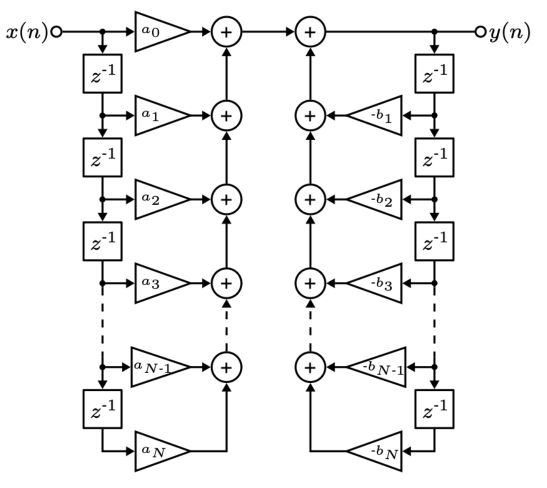
\includegraphics[width=0.5\textwidth]{Images/Type-1.png}
\end{center}
\subsubsection{Type 2}
$$y(n)=\sum_{i=0}^{N}a_{i}x(n-i)-\sum_{i=1}^{N}b_{i}y(n-i)$$
\begin{center}
  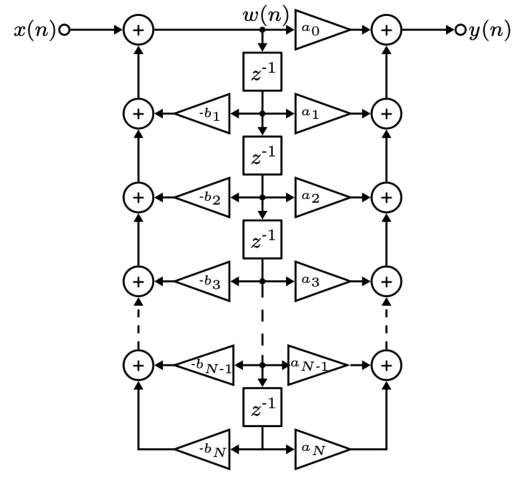
\includegraphics[width=0.5\textwidth]{Images/Type-2.png}
\end{center}
\subsection{Cascade and Parallel Realization}
A higher-order system can be implemented as a cascade of $M$ sections given as follows:
$$H(z)=H_1(z)\cdot H_2(z)\cdot H_3(z)\cdot \dots \cdot H_M(z)\cdot$$

A higher-order system can be implemented as a parallel realization of transfer functions that are a 1st-order or 2nd-order transfer function. These transfer functions are found by partial fraction resolution of $H(z)$.
$$H(z)=C+H_1(z)+H_2(z)+\dots+H_M(z)$$
